\begin{figure}[] \centering
	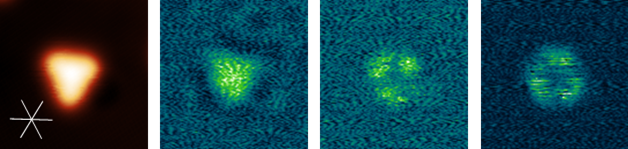
\includegraphics[width=0.7\textwidth]{./images/hbbnc-maps}
	\caption{Choosing the spectroscopy energy to match one of the spectral maxima of the line spectra reveals the spatial distribution of electronic states as shown in the STS map. While at 650 meV only the core contributes to the DOS, energies of 1200 meV and 1600 meV are located on the leg and edge positions respectively.}
	\label{}
\end{figure}

\begin{figure}[] \centering
	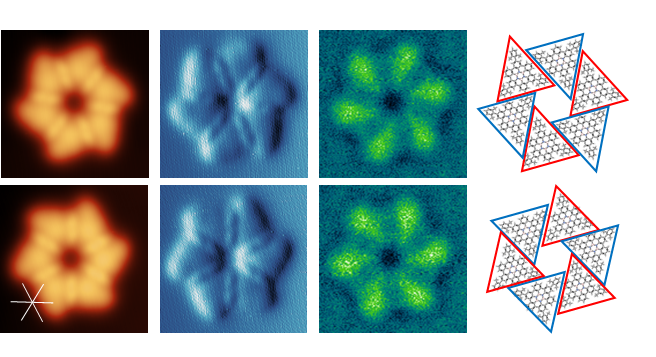
\includegraphics[width=0.7\textwidth]{./images/hbbnc-maps2}
	\caption{Comparison of two hexamers (chiral twins). While in STM the most apparent change is the orientation of the molecules within the hexamer and the resulting change in the protrusion between them, dI/dV maps (600 meV) clearly highlight the turn direction within the hexamer.}
	\label{}
\end{figure}

\begin{figure}[] \centering
	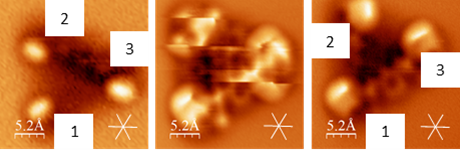
\includegraphics[width=0.7\textwidth]{./images/hbbnc-ag-111-leg-flip}
	\caption{Conformational change of a monomer after several scans with the AFM. First the molecule starts with an orientation of the legs in 1: clockwise, 2: counterclockwise, 3: clockwise. After several scans in close proximity (how far?!) legs at positions 2 and 3 flip around and change their orientation to 1: clockwise, 2: clockwise, 3: counterclockwise. This results in a changed adsorption geometry. First the upper right edge is lifted from the substrate, while after the leg rearrangement the lower right edge is lifted from the surface. This is caused by the lower lying dimethyl groups lifting the phenyl ring and the molecules edge.}
	\label{}
\end{figure}

\begin{figure}[] \centering
	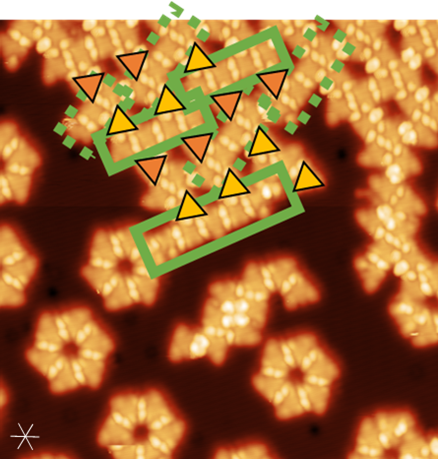
\includegraphics[width=0.7\textwidth]{./images/hbbnc-ag-111-rt-med-coverage-spacer-mol}
	\caption{Rows are separated by two sets of spacer molecules (orange/yellow). 
		\textcolor{red}{\textbf{What is their position in the unit cell? Rotation? Separation to all the other molecules?}}
	}
	\label{}
\end{figure}

